\documentclass[11pt]{article}
\usepackage{geometry,marginnote} % Pour passer au format A4
\geometry{hmargin=1cm, vmargin=1cm} % 

% Page et encodage
\usepackage[T1]{fontenc} % Use 8-bit encoding that has 256 glyphs
\usepackage[english,french]{babel} % Français et anglais
\usepackage[utf8]{inputenc} 

\usepackage{lmodern,numprint}
\setlength\parindent{0pt}

% Graphiques
\usepackage{graphicx,float,grffile,units}
\usepackage{tikz,pst-eucl,pst-plot,pstricks,pst-node,pstricks-add,pst-fun} 

% Maths et divers
\usepackage{amsmath,amsfonts,amssymb,amsthm,verbatim}
\usepackage{multicol,enumitem,url,eurosym,gensymb,tabularx}

\DeclareUnicodeCharacter{20AC}{\euro}



% Sections
\usepackage{sectsty} % Allows customizing section commands
\allsectionsfont{\centering \normalfont\scshape}

% Tête et pied de page
\usepackage{fancyhdr} \pagestyle{fancyplain} \fancyhead{} \fancyfoot{}

\renewcommand{\headrulewidth}{0pt} % Remove header underlines
\renewcommand{\footrulewidth}{0pt} % Remove footer underlines

\newcommand{\horrule}[1]{\rule{\linewidth}{#1}} % Create horizontal rule command with 1 argument of height

\newcommand{\Pointilles}[1][3]{%
  \multido{}{#1}{\makebox[\linewidth]{\dotfill}\\[\parskip]
}}

\newtheorem{Definition}{Définition}

\usepackage{siunitx}
\sisetup{
    detect-all,
    output-decimal-marker={,},
    group-minimum-digits = 3,
    group-separator={~},
    number-unit-separator={~},
    inter-unit-product={~}
}

\setlength{\columnseprule}{1pt}

\begin{document}

\textbf{Nom, Prénom :} \hspace{8cm} \textbf{Classe :} \hspace{3cm} \textbf{Date :}\\

\begin{center}
  \textit{La plus coûteuse des dépenses, c’est la perte de temps.}  - \textbf{Théophraste}
\end{center}

\subsection*{Restituer les connaissances}

\begin{enumerate}
  \item[1.] Propriété : La somme des angles. \newline \Pointilles[1]
  \item[2.] Définition : Triangles semblables. \newline \Pointilles[1]
  \item[3.] Propriété : Les côtés des triangles semblables. \newline \Pointilles[1]
\end{enumerate}

\subsection*{ex1a - Calculer les angles dans les triangles}
\textbf{(modéliser, écrire le calcul, calculer)}

\begin{figure}[H]
  \centering
  \includegraphics[width=0.55\linewidth]{4x3-triangles-semblables/ie-ex1a.pdf}
\end{figure}
\Pointilles[2]

\begin{minipage}[t]{0.55\textwidth}
  \subsection*{ex1b - Calculer l'angle}
  \textbf{(justifier, écrire les calculs, calculer)}
  \Pointilles[6]
\end{minipage}
\begin{minipage}[t]{0.4\textwidth}
  \begin{figure}[H]
    \centering
    \includegraphics[width=0.6\linewidth]{4x3-triangles-semblables/ie-ex2a.pdf}
  \end{figure}
\end{minipage}

\begin{minipage}[t]{0.55\textwidth}
  \subsection*{ex2 - Démontrer}
  \textit{Démontrer que les triangles ABC, AHB et BHC sont semblables}
  \textbf{(justifier, écrire les calculs, conclure)}
  \begin{figure}[H]
    \centering
    \includegraphics[width=0.7\linewidth]{4x3-triangles-semblables/ie-ex3a.pdf}
  \end{figure}
\end{minipage}
\begin{minipage}[t]{0.4\textwidth}
  \Pointilles[14]
\end{minipage}

\newpage

\subsection*{ex3 - Calculer les longueurs dans les triangles semblables}
\textbf{(justifier, écrire le tableau, écrire les calculs, calculer)} \newline
\begin{minipage}[t]{0.45\textwidth}
  \textit{Les triangles 1 et 2 sont semblables.} 
  \begin{figure}[H]
    \centering
    \includegraphics[width=0.6\linewidth]{4x3-triangles-semblables/ie-ex4a.pdf}
  \end{figure}
\end{minipage}
\begin{minipage}[t]{0.55\textwidth}
  \begin{tabular}{|c|c|c|c|}
    \hline
    \phantom{$\dfrac{azerty}{1}$} & \phantom{azerty}  & \phantom{azerty} & \phantom{azerty} \\ \hline
    \phantom{$\dfrac{azerty}{1}$} & \phantom{azerty}  & \phantom{azerty} & \phantom{azerty} \\   \hline
  \end{tabular}

  \Pointilles[6]
\end{minipage}


\subsection*{Les petits problèmes}
\textbf{Il faut résoudre et rédiger les problèmes suivants sur feuille :} 

\begin{minipage}[t]{0.3\textwidth}
  \begin{figure}[H]
    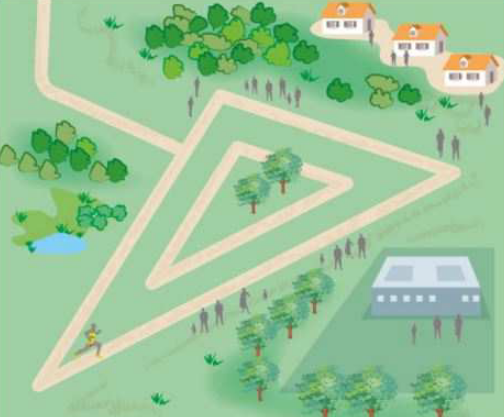
\includegraphics[width=0.7\linewidth]{4x3-triangles-semblables/ie-pb1.png}
  \end{figure}
\end{minipage}
\begin{minipage}[t]{0.65\textwidth}
  \subsection*{pb1 - Course à pied}

  Dans un parc, deux circuits forment deux triangles semblables. Les dimensions des côtés du petit circuit sont $320m$, $380m$ et $590m$. Le petit côté du grand circuit mesure $400 m$.

  \textbf{Quelle distance parcourt Ahmet quand elle effectue cinq tours du grand circuit ?}
\end{minipage}

\horrule{1px}

\begin{minipage}[t]{0.5\textwidth}
  \begin{figure}[H]
    \includegraphics[width=0.8\linewidth]{4x3-triangles-semblables/ie-pb2.pdf}
  \end{figure}
\end{minipage}
\begin{minipage}[t]{0.45\textwidth}
  \subsection*{pb2 - Tour Eiffel}

  Pour estimer la hauteur de la tour Eiffel à Paris, votre professeur d'une taille TL=1,94m pose un miroir à une distance TM=1m de lui dans lequel il arrive à voir le sommet de la tour. 

\textbf{Calculer la hauteur de la tour.}
\end{minipage}

\horrule{1px}

\begin{minipage}[t]{0.2\textwidth}
  \begin{figure}[H]
    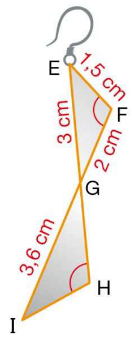
\includegraphics[width=0.6\linewidth]{4x3-triangles-semblables/ie-pb3.png}
  \end{figure}
\end{minipage}
\begin{minipage}[t]{0.75\textwidth}
  \subsection*{pb3 - Boucle d'oreille}

  Sofiane souhaite acheter des boucles d'oreille sa fille. Les triangles EFG et IHG sont semblables. 1cm d'Or coûte 55€. Il achète deux boucles d'oreille.  

\textbf{Après avoir calculer la longueur du fil d'or, calculer le prix du cadeau. }
\end{minipage}

\newpage

\textbf{Nom, Prénom :} \hspace{8cm} \textbf{Classe :} \hspace{3cm} \textbf{Date :}\\

\begin{center}
  \textit{La plus coûteuse des dépenses, c’est la perte de temps.}  - \textbf{Théophraste}
\end{center}

\subsection*{Restituer les connaissances}

\begin{enumerate}
  \item[1.] Propriété : La somme des angles. \newline \Pointilles[1]
  \item[2.] Définition : Triangles semblables. \newline \Pointilles[1]
  \item[3.] Propriété : Les côtés des triangles semblables. \newline \Pointilles[1]
\end{enumerate}

\subsection*{ex1a - Calculer les angles dans les triangles}
\textbf{(modéliser, écrire le calcul, calculer)}

\begin{figure}[H]
  \centering
  \includegraphics[width=0.55\linewidth]{4x3-triangles-semblables/ie-ex1b.pdf}
\end{figure}
\Pointilles[2]

\begin{minipage}[t]{0.55\textwidth}
  \subsection*{ex1b - Calculer l'angle}
  \textbf{(justifier, écrire les calculs, calculer)}
  \Pointilles[6]
\end{minipage}
\begin{minipage}[t]{0.4\textwidth}
  \begin{figure}[H]
    \centering
    \includegraphics[width=0.6\linewidth]{4x3-triangles-semblables/ie-ex2b.pdf}
  \end{figure}
\end{minipage}

\begin{minipage}[t]{0.55\textwidth}
  \subsection*{ex2 - Démontrer}
  \textit{Démontrer que les triangles ABC, AHB et BHC sont semblables}
  \textbf{(justifier, écrire les calculs, conclure)}
  \begin{figure}[H]
    \centering
    \includegraphics[width=0.7\linewidth]{4x3-triangles-semblables/ie-ex3b.pdf}
  \end{figure}
\end{minipage}
\begin{minipage}[t]{0.4\textwidth}
  \Pointilles[14]
\end{minipage}

\newpage

\subsection*{ex3 - Calculer les longueurs dans les triangles semblables}
\textbf{(justifier, écrire le tableau, écrire les calculs, calculer)} \newline
\begin{minipage}[t]{0.45\textwidth}
  \textit{Les triangles 1 et 2 sont semblables.} 
  \begin{figure}[H]
    \centering
    \includegraphics[width=0.6\linewidth]{4x3-triangles-semblables/ie-ex4b.pdf}
  \end{figure}
\end{minipage}
\begin{minipage}[t]{0.55\textwidth}
  \begin{tabular}{|c|c|c|c|}
    \hline
    \phantom{$\dfrac{azerty}{1}$} & \phantom{azerty}  & \phantom{azerty} & \phantom{azerty} \\ \hline
    \phantom{$\dfrac{azerty}{1}$} & \phantom{azerty}  & \phantom{azerty} & \phantom{azerty} \\   \hline
  \end{tabular}

  \Pointilles[6]
\end{minipage}


\subsection*{Les petits problèmes}
\textbf{Il faut résoudre et rédiger les problèmes suivants sur feuille :} 

\begin{minipage}[t]{0.3\textwidth}
  \begin{figure}[H]
    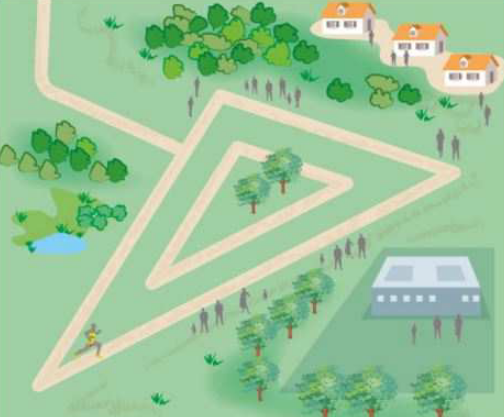
\includegraphics[width=0.7\linewidth]{4x3-triangles-semblables/ie-pb1.png}
  \end{figure}
\end{minipage}
\begin{minipage}[t]{0.65\textwidth}
  \subsection*{pb1 - Course à pied}

  Dans un parc, deux circuits forment deux triangles semblables. Les dimensions des côtés du petit circuit sont $310m$, $360m$ et $580m$. Le petit côté du grand circuit mesure $400 m$.

  \textbf{Quelle distance parcourt Ahmet quand elle effectue cinq tours du grand circuit ?}
\end{minipage}

\horrule{1px}

\begin{minipage}[t]{0.5\textwidth}
  \begin{figure}[H]
    \includegraphics[width=0.8\linewidth]{4x3-triangles-semblables/ie-pb2.pdf}
  \end{figure}
\end{minipage}
\begin{minipage}[t]{0.45\textwidth}
  \subsection*{pb2 - Tour Eiffel}

  Pour estimer la hauteur de la tour Eiffel à Paris, votre professeur d'une taille TL=1,92m pose un miroir à une distance TM=1m de lui dans lequel il arrive à voir le sommet de la tour. 

\textbf{Calculer la hauteur de la tour.}
\end{minipage}

\horrule{1px}

\begin{minipage}[t]{0.2\textwidth}
  \begin{figure}[H]
  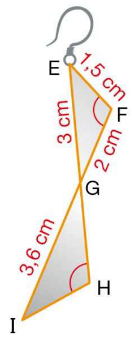
\includegraphics[width=0.6\linewidth]{4x3-triangles-semblables/ie-pb3.png}
  \end{figure}
\end{minipage}
\begin{minipage}[t]{0.75\textwidth}
  \subsection*{pb3 - Boucle d'oreille}

  Sofiane souhaite acheter des boucles d'oreille sa fille. Les triangles EFG et IHG sont semblables. 1cm d'Or coûte 54€. Il achète deux boucles d'oreille.  

\textbf{Après avoir calculer la longueur du fil d'or, calculer le prix du cadeau. }
\end{minipage}

\end{document}